\chapter{回归分析}

\section{线性回归}

假如有下列 excel 表格的数据:

\begin{figure}[ht]
  \centering
  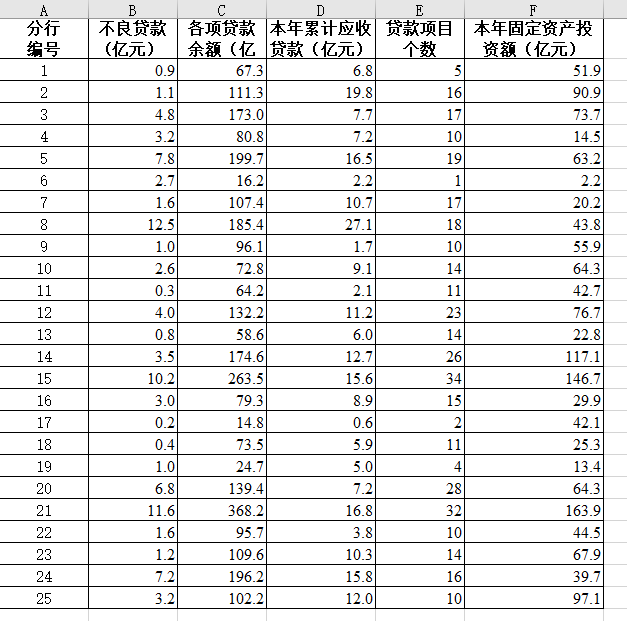
\includegraphics{figure/linear_regression.png}
\end{figure}

该文件以 lienar\_regression.xlsx 存到电脑上,我们首先用 pandas 包读取该 excel 数据,

\begin{lstlisting}[Language=Python]
>>> import pandas as pd
>>> datas = pd.read_excel(r'D:\Users\chen_\git\Statistics-book\datas\linear_regression.xlsx') # 读取 excel 数据,引号里面是 excel 文件在电脑的存储位置
>>> datas.head() # 显示 excel 数据文件的前 5 行数据
   分行\n编号  不良贷款(亿元)  各项贷款余额(亿元)  本年累计应收贷款(亿元)  贷款项目个数(个)  本年固定资产投资额(亿元)
0       1       0.9        67.3           6.8          5           51.9
1       2       1.1       111.3          19.8         16           90.9
2       3       4.8       173.0           7.7         17           73.7
3       4       3.2        80.8           7.2         10           14.5
4       5       7.8       199.7          16.5         19           63.2

\end{lstlisting}

\subsection{线性回归}

使用 python 做线性回归分析有好几种方式,常用的分别是 scipy 包(只能做一元线性回归),statsmodels 包,以及 sklearn 包。但是,\textcolor{red}{这些包目前都不能处理共线性,即自动剔除部分共线性的变量},这需要自己去编写相应函数。

\subsubsection{使用 scipy 包}

scipy.stats 中的 linregress 函数可以做一元线性回归。假如因变量为 “不良贷款”,自变量为 “各项贷款余额”,全部 python 代码如下:

\begin{lstlisting}[Language=Python]
import scipy.stats as st
import pandas as pd

datas = pd.read_excel(r'D:\Users\chen_\git\Statistics-book\datas\linear_regression.xlsx') # 读取 excel 数据,引号里面是 excel 文件的位置
y = datas.iloc[:, 1] # 因变量为第 2 列数据
x = datas.iloc[:, 2] # 自变量为第 3 列数据

# 线性拟合,可以返回斜率,截距,r 值,p 值,标准误差
slope, intercept, r_value, p_value, std_err = st.linregress(x, y)

print(slope)# 输出斜率
print(intercept) # 输出截距
print(r_value**2) # 输出 R^2
\end{lstlisting}


scipy 中的回归分析比较简单,目前只能做一元线性回归,也不能用来做预测。

\subsubsection{使用 statsmodel 包}

使用 statsmodel 包中的 OLS (普通最小二乘法)函数,可以构建统计模型,并进行线性拟合。假如因变量为 “不良贷款”,自变量为 “各项贷款余额”,则构建最小二乘的模型以及回归分析的代码如下:

\begin{lstlisting}[Language=Python]
>>> import statsmodels.api as sm
>>> y = datas.iloc[:, 1] # 因变量为第 2 列数据
>>> x = datas.iloc[:, 2] # 自变量为第 3 列数据
>>> x = sm.add_constant(x) # 若模型中有截距,必须有这一步
>>> model = sm.OLS(y, x).fit() # 构建最小二乘模型并拟合
>>> print(model.summary()) # 输出回归结果
\end{lstlisting}

回归结果如下图所示:

\begin{figure}[ht]
  \centering
  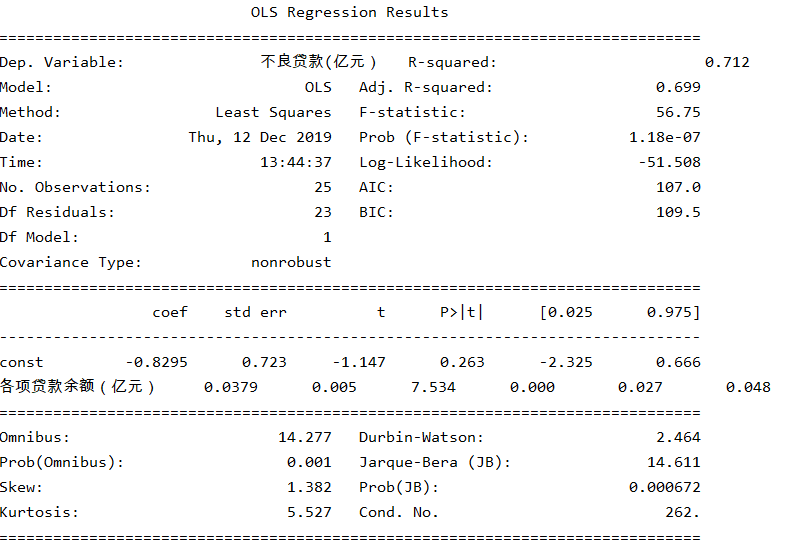
\includegraphics[scale=0.8]{figure/linearRegressionResult.png}
\end{figure}

若要画出实际数据与预测图形,可以加上下面代码:

\begin{lstlisting}[Language=Python]
# 画图
# 这两行代码在画图时添加中文必须用
>>> plt.rcParams['font.sans-serif'] = ['SimHei']
>>> plt.rcParams['axes.unicode_minus'] = False

>>> predicts = model.predict() # 模型的预测值
>>> x = datas.iloc[:, 2] # 自变量为第 3 列数据
>>> plt.scatter(x, y, label='实际值') # 散点图
>>> plt.plot(x, predicts, color = 'red', label='预测值')
>>> plt.legend() # 显示图例,即每条线对应 label 中的内容
>>> plt.show() # 显示图形
\end{lstlisting}

图形:

\begin{figure}[ht]
  \centering
  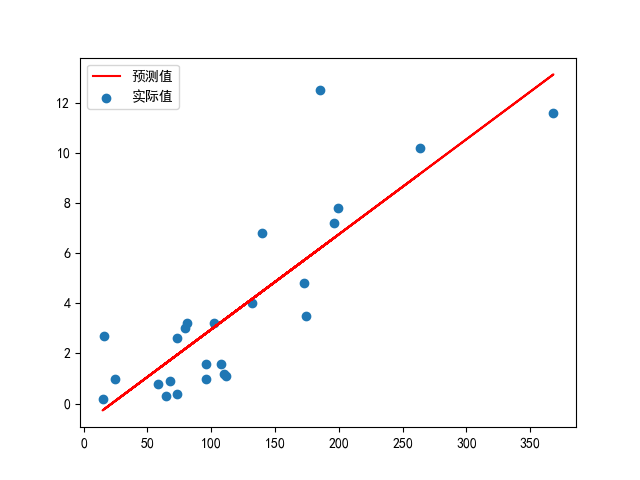
\includegraphics[scale=0.5]{figure/lineRegression1.png}
\end{figure}

全部 python 代码如下:

\begin{lstlisting}[Language=Python]
import pandas as pd
import statsmodels.api as sm
import matplotlib.pyplot as plt

datas = pd.read_excel(r'D:\Users\chen_\git\Statistics-book\datas\linear_regression.xlsx') # 读取 excel 数据,引号里面是 excel 文件的位置
y = datas.iloc[:, 1] # 因变量为第 2 列数据
x = datas.iloc[:, 2] # 自变量为第 3 列数据
x = sm.add_constant(x) # 若模型中有截距,必须有这一步
model = sm.OLS(y, x).fit() # 构建最小二乘模型并拟合
print(model.summary()) # 输出回归结果

# 画图
# 这两行代码在画图时添加中文必须用
plt.rcParams['font.sans-serif'] = ['SimHei']
plt.rcParams['axes.unicode_minus'] = False

predicts = model.predict() # 模型的预测值
x = datas.iloc[:, 2] # 自变量为第 3 列数据
plt.scatter(x, y, label='实际值') # 散点图
plt.plot(x, predicts, color = 'red', label='预测值')
plt.legend() # 显示图例,即每条线对应 label 中的内容
plt.show() # 显示图形
\end{lstlisting}

注意:若导入包时使用命令 import statsmodels.formula.api as sm, 则在回归分析时不用添加截距 add\_constant,但是必须使用统计语言给出模型信息,代码如下:

\begin{lstlisting}[Language=Python]
import pandas as pd
import statsmodels.formula.api as sm
import matplotlib.pyplot as plt

datas = pd.read_excel(r'D:\Users\chen_\git\Statistics-book\datas\linear_regression.xlsx') # 读取 excel 数据,引号里面是 excel 文件的位置
model = sm.ols('不良贷款~各项贷款余额', datas).fit() # 构建最小二乘模型并拟合,
                               #此时不用单独输入 x,y了,而是将自变量与因变量用统计语言公式表示,将全部数据导入
print(model.summary()) # 输出回归结果


# 画图
# 这两行代码在画图时添加中文必须用
plt.rcParams['font.sans-serif'] = ['SimHei']
plt.rcParams['axes.unicode_minus'] = False

predicts = model.predict() # 模型的预测值
y = datas.iloc[:, 1] # 因变量为第 2 列数据
x = datas.iloc[:, 2] # 自变量为第 3 列数据
plt.scatter(x, y, label='实际值')
plt.plot(x, predicts, color = 'red', label='预测值')
plt.legend() # 显示图例,即每条线对应 label 中的内容
plt.show() # 显示图形
\end{lstlisting}

在多元回归中,只需把自变量改为多列数据即可,假如不良贷款为因变量,从第3列到第6列都是因变量,则使用 statsmodels 包的全部 python 代码如下:

\begin{lstlisting}[Language=Python]
import pandas as pd
import statsmodels.api as sm
import matplotlib.pyplot as plt

datas = pd.read_excel(r'D:\Users\chen_\git\Statistics-book\datas\linear_regression.xlsx') # 读取 excel 数据,引号里面是 excel 文件的位置
y = datas.iloc[:, 1] # 因变量为第 2 列数据
x = datas.iloc[:, 2:6] # 自变量为第 3 列到第 6 列数据
x = sm.add_constant(x) # 若模型中有截距,必须有这一步
model = sm.OLS(y, x).fit() # 构建最小二乘模型并拟合
print(model.summary()) # 输出回归结果
\end{lstlisting}

统计结果图如下:

\begin{figure}[ht]
  \centering
  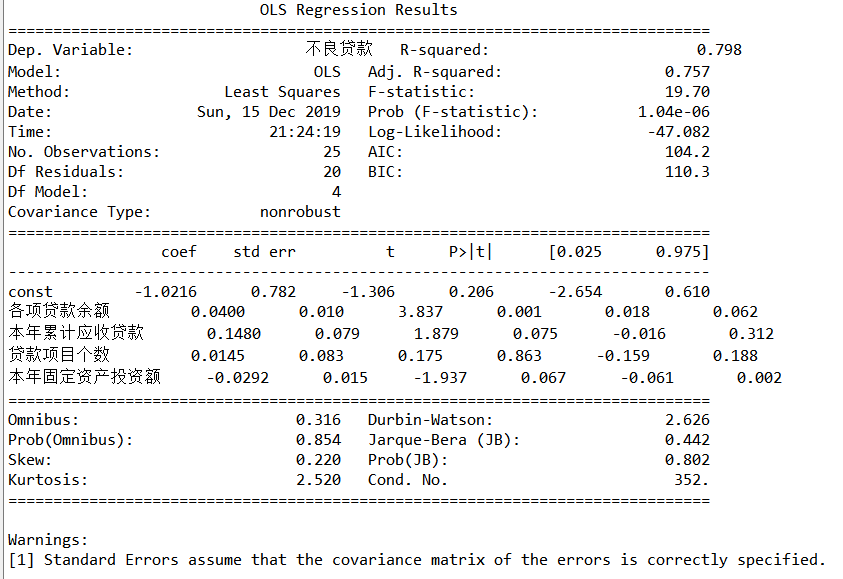
\includegraphics[scale=0.8]{figure/linearRegressionResult2.png}
\end{figure}




\subsubsection{使用 sklearn 包}

sklearn 包机器学习中常见的 python 包,可以用来做统计分析时,但它并不能像 statsmodels 那样生成非常详细的统计分析结果。一元回归时,自变量与因变量都需要处理下,对于上面同样的例子:

\begin{lstlisting}[Language=Python]
import pandas as pd
import matplotlib.pyplot as plt
import numpy as np
from sklearn.linear_model import LinearRegression

datas = pd.read_excel(r'D:\Users\chen_\git\Statistics-book\datas\linear_regression.xlsx') # 读取 excel 数据,引号里面是 excel 文件的位置
y = datas.iloc[:, 1] # 因变量为第 2 列数据
x = datas.iloc[:, 2] # 自变量为第 3 列数据

# 将 x,y 分别增加一个轴,以满足 sklearn 中回归模型认可的数据
x = x[:, np.newaxis]
y = y[:, np.newaxis]

model = LinearRegression() # 构建线性模型
model.fit(x, y) # 自变量在前,因变量在后
predicts = model.predict(x) # 预测值
R2 = model.score(x, y) # 拟合程度 R2
print('R2 = %.2f' % R2) # 输出 R2
coef = model.coef_ # 斜率
intercept = model.intercept_ # 截距
print(model.coef_, model.intercept_) # 输出斜率和截距

# 画图
plt.rcParams['font.sans-serif'] = ['SimHei']
plt.rcParams['axes.unicode_minus'] = False

y = datas.iloc[:, 1] # 因变量为第 2 列数据
x = datas.iloc[:, 2] # 自变量为第 3 列数据
plt.scatter(x, y, label='实际值') # 散点图
plt.plot(x, predicts, color = 'red', label='预测值')
plt.legend() # 显示图例,即每条线对应 label 中的内容
plt.show() # 显示图形
\end{lstlisting}


用 sklearn 做多元回归时,全部代码如下:
\begin{lstlisting}[Language=Python]
import pandas as pd
import matplotlib.pyplot as plt
import numpy as np
from sklearn.linear_model import LinearRegression

datas = pd.read_excel(r'D:\Users\chen_\git\Statistics-book\datas\linear_regression.xlsx') # 读取 excel 数据,引号里面是 excel 文件的位置
y = datas.iloc[:, 1] # 因变量为第 2 列数据
x = datas.iloc[:, 2:6] # 自变量为第 3 列到第 6 列数据

# 将 y 分别增加一个轴,以满足 sklearn 中回归模型认可的数据
# 此时由于 x 是多元变量,则不用添加新的轴了
y = y[:, np.newaxis]

model = LinearRegression() # 构建线性模型
model.fit(x, y) # 自变量在前,因变量在后
predicts = model.predict(x) # 预测值
R2 = model.score(x, y) # 拟合程度 R2
print('R2 = %.3f' % R2) # 输出 R2
coef = model.coef_ # 斜率
intercept = model.intercept_ # 截距
print(model.coef_, model.intercept_) # 输出斜率和截距
\end{lstlisting}



\subsubsection{共线性}

\subsection{多项式回归}

对于一些曲线型数据,一般通过拟合成多项式函数回归。从 2009 年到2018年阿里巴巴公布的历年销售额数据如下:

\begin{table}[!ht]
\centering
\begin{tabular}{|l|r|}
\hline

年份 & 销量 \\ \hline
2009 & 0.5 \\ \hline
2010 & 9.36 \\ \hline
2011 & 52 \\ \hline
2012 & 191 \\ \hline
2013 & 350 \\ \hline
2014 & 571 \\ \hline
2015 & 912 \\ \hline
2016 & 1207 \\ \hline
2017 & 1682.69 \\ \hline
2018 & 2135 \\ \hline

\end{tabular}
\end{table}

首先画出折线图,观察一下数据的趋势规律:

\begin{lstlisting}[Language=Python]
import numpy as np
import matplotlib.pyplot as plt


sales_datas = [0.5, 9.36, 52, 191, 350, 571, 912, 1207, 1682.69, 2135]
year = np.arange(2009, 2019)

# 画图
# 这两行代码使得 pyplot 画出的图形中可以显示中文
plt.rcParams['font.sans-serif'] = ['SimHei']
plt.rcParams['axes.unicode_minus'] = False

plt.plot(year, sales_datas, 'o-', label = '公布销售额') # 折线图
plt.legend() # 显示图例, 图例中内容由 label 定义
plt.show()
\end{lstlisting}

\begin{figure}[ht]
  \centering
  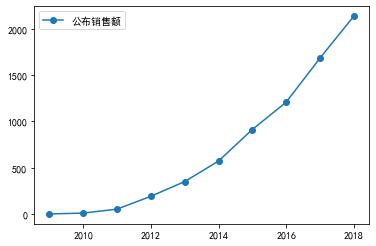
\includegraphics[scale=0.8]{figure/polyRegression1.png}
\end{figure}

从图像上看,数据的折线图非常类似一个多项式曲线,因此我们可以做多项式回归。

\subsubsection{使用 Numpy}

Numpy 包的 polyfit 函数可以实现对数据的多项式回归,然后通过 poly1d 函数将多项式拟合的参数值生成多项式函数,全部拟合代码如下:

\begin{lstlisting}[Language=Python]
import numpy as np
import matplotlib.pyplot as plt


sales_datas = [0.5, 9.36, 52, 191, 350, 571, 912, 1207, 1682.69, 2135]
year = np.arange(2009, 2019)
year_num = np.arange(1, 11)

# 画图
# 这两行代码使得 pyplot 画出的图形中可以显示中文
plt.rcParams['font.sans-serif'] = ['SimHei']
plt.rcParams['axes.unicode_minus'] = False

plt.plot(year, sales_datas, 'o-', label = '公布销售额') # 折线图


# 拟合
fit_parameters = np.polyfit(year_num, sales_datas, 3) # 拟合成三次方
forecast_function = np.poly1d(fit_parameters)  # 预测(拟合)的函数

# 预测
forecast2019 = forecast_function(11) # 2019 是第11年
print(forecast2019) # 输出 2019 年的预测结果

forecasts = forecast_function(np.arange(1, 12))
plt.plot(np.append(year, 2019), forecasts, 'o:', label='预测销量')
plt.legend() # 显示图例, 图例中内容由 label 定义
plt.show()
\end{lstlisting}

\begin{figure}[ht]
  \centering
  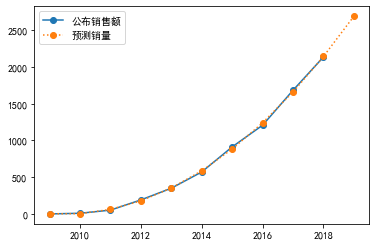
\includegraphics[scale=0.8]{figure/polyRegression2.png}
\end{figure}

\section{非线性回归}
